% Homework report template for courses lectured by Blaz Zupan.
% For more on LaTeX please consult its documentation pages, or
% read tutorials like http://tobi.oetiker.ch/lshort/lshort.pdf.
%
% Use pdflatex to produce a PDF of a report.

\documentclass[a4paper,11pt]{article}
\usepackage{a4wide}
\usepackage{fullpage}
\usepackage[toc,page]{appendix}
\usepackage[pdftex]{graphicx} % for figures
\usepackage{setspace}
\usepackage{color}
\definecolor{light-gray}{gray}{0.95}
\usepackage{listings} % for inclusion of Python code
\usepackage{hyperref}
\renewcommand{\baselinestretch}{1.2}

\lstset{ % style for Python code, improve if needed
    language=Python,
    basicstyle=\footnotesize,
    basicstyle=\ttfamily\footnotesize\setstretch{1},
    backgroundcolor=\color{light-gray},
}

\title{Gene Prediction}
\author{Miha Zidar (63060317)}
\date{\today}

\begin{document}

\maketitle

\section{Introduction}

In this homework we look at a basic prediction of open reading frames (from now ORFs) in \textit{Paramecium tetraurelia} and \textit{Emiliania huxleyi virus 86}. We also test how good the most simple predicting algorithm works.

\section{Data}

Data for this homework was retrieved from a gene bank with BioPython. We used genome sequences for \textit{Paramecium tetraurelia (NC\_006058)} and \textit{Emiliania huxleyi virus 86 (NC\_007346)}. Loaded data cotains the seqence and all known features of the genome with some usefull functions for manipulating the sequence. We used downloaded genome features to test the precision and recall of our algorithm.


\section{Methods}

\subsection{Detecting ORFs}
All genomes contains many ORFs. An ORF is determened by a start codon and a stop codon. Our algorithm will have to match start and stop codons so that the folowing will hold:
\begin{itemize}
    \item start and stop codon have to be aligned so that there are only multiples of three codons between. 
    \item if we have multiple possible start codons, we'll choose the one that gives us the longest ORF.
    \item there should not be any alinged stop codons between a start and a stop codon of an ORF.
    \item we have to repeat the search on the reverse complement sequence. 
\end{itemize}
ORFs may overlap but only if they are not aligned, if they're on the reverse strand of the genome.

\subsection{Precission and recall}
To assess the ORF predictions of our algorithm, we will take a look at precission and recall, and how those change when we limit our results with a certain lenght. These two mesurements are defined as:
\[
    Precision = \frac{TruePositives }{TruePositives + FalsePositives}
\]
\[
    Recall = \frac{TruePositives }{TruePositives + FalseNegatives}
\]

\subsection{Area under PR-curve}

If we plot precission as a function of Recall \ref{prcurve}, we could compare the surface area unded the curve with some other algorithm. It can bs shown that this kind of comparison will usually yield better results than a simmilar AUC score. 


\section{Results}


\begin{table}[htbp]
    \caption{Some basic data for both genomes.}
    \label{tab1}
    \begin{center}
        \begin{tabular}{ l | c | r }
            \hline                        
            & NC\_006058 & NC\_007346 \\
            \hline                        
            \# of real ORFs & 463 & 472 \\
            \hline                        
            \# of predicted ORFs & 16646 & 18088 \\
            \hline                        
            average length & 548.03 & 261.70 \\
            \hline  
            average predicted length & 59.75 & 27.09 \\
            \hline  
            \# of predicted ORFs longer than 60 & 5174 & 1469 \\
            \hline  
            precision for at least 125 codons: & 0.10087 & 0.67811 \\
            \hline  
            recall for at least 125 codons & 0.40172 & 0.66949 \\
            \hline  
            area under PR-curve & 0.10785 & 0.60254 \\
            \hline  

        \end{tabular}
    \end{center}
\end{table}

The second genome, has more start and stop codons, and that meakes it easy to match a vampire from a human, since the average ORF length is half as small. 



\begin{figure}[htbp]
    \begin{center}
        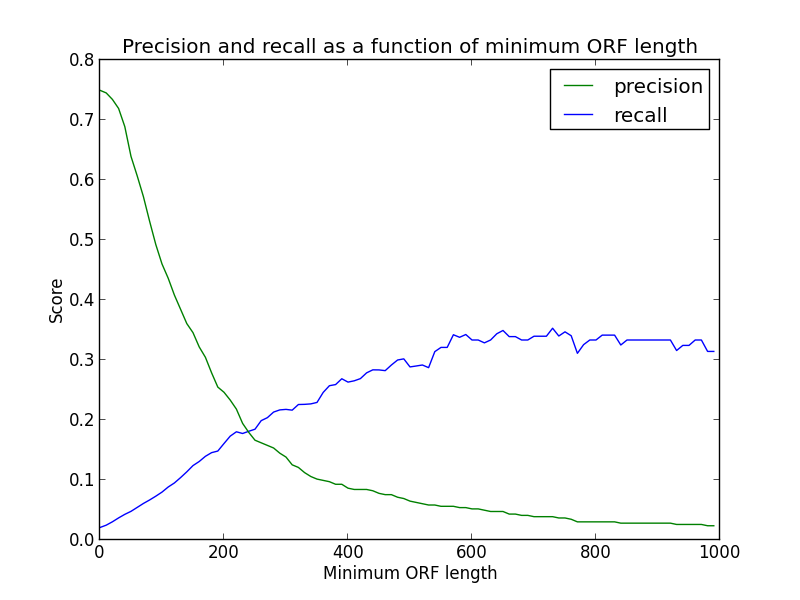
\includegraphics[scale=0.6]{src/precision_recall-NC_006058.png}
        \caption{Precission and Recall as they depend on the minimum ORF legth for NC\_006058}
        \label{fig-example}
    \end{center}
\end{figure}

\begin{figure}[htbp]
    \begin{center}
        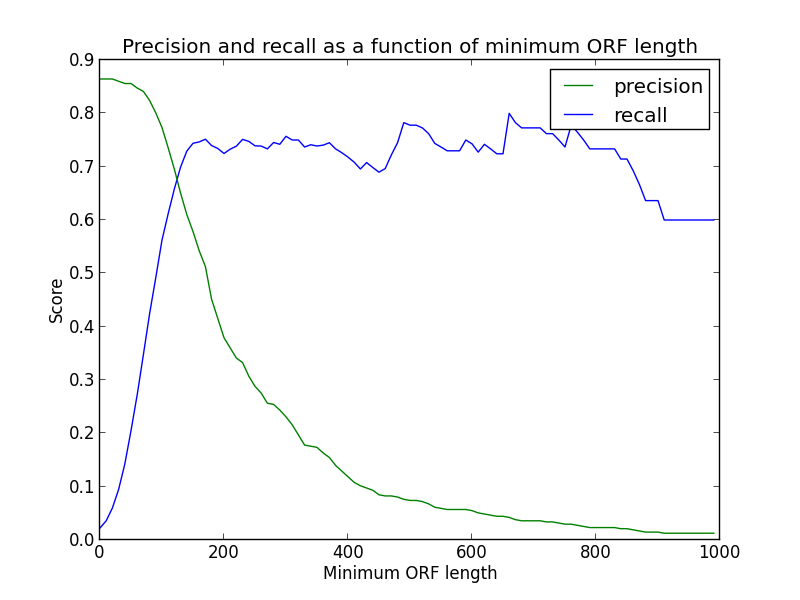
\includegraphics[scale=0.6]{src/precision_recall-NC_007346.png}
        \caption{Precission and Recall as they depend on the minimum ORF legth for NC\_007346}
        \label{fig-example}
    \end{center}
\end{figure}

\begin{figure}[htbp]
    \begin{center}
        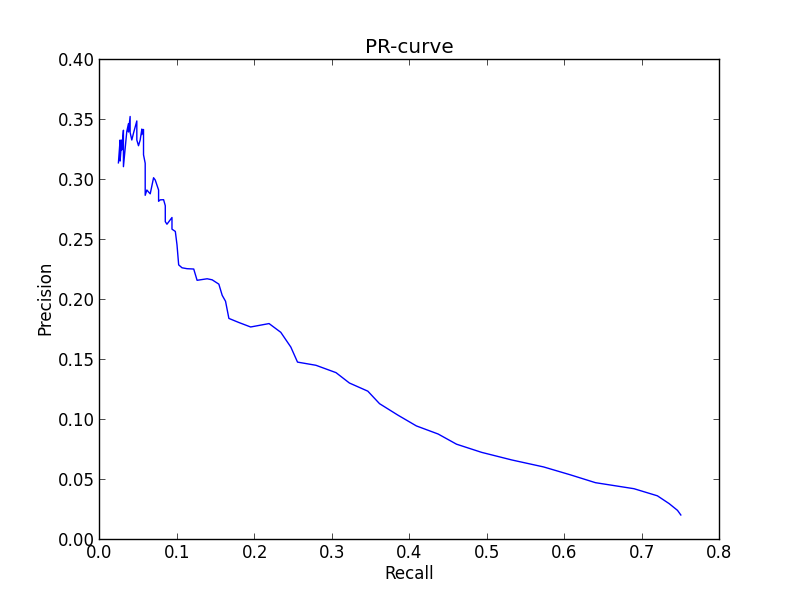
\includegraphics[scale=0.6]{src/PR-curve-NC_006058.png}
        \caption{PR-curve from which we'll calculate the area under the curve for NC\_006058}
        \label{prcurve}
    \end{center}
\end{figure}





\subsection*{Honor Code}

% The following paragraph of your report should be included as is - do % not change it.

My answers to homework are my own work. I did not make solutions or code available to anyone else. I did not engage in any other activities that will dishonestly improve my results or dishonestly improve/hurt the results of others.

\end{document}

